\documentclass[11pt]{amsart}

\usepackage{geometry}
\usepackage{showlabels}
\usepackage{caption}
\usepackage{multirow}
\usepackage{hyperref}
\usepackage{algpseudocode}
\usepackage{todonotes}
\usepackage[noline,ruled]{algorithm2e}
\usepackage{enumerate}
\usepackage{graphicx}
%\setlength{\parindent}{0pt}
\geometry{
  includeheadfoot,
  margin=2.54cm
}

\setcounter{tocdepth}{1}

\makeatletter
\def\imod#1{\allowbreak\mkern10mu({\operator@font mod}\,\,#1)}
\makeatother

\newtheorem*{problem}{Problem}
\theoremstyle{definition}
\newtheorem*{answer}{Answer}

\newcommand{\R}{\mathbb{R}}
\newcommand{\D}{\mathcal{D}}
\newcommand{\N}{\mathbb{N}}
\newcommand{\Z}{\mathbb{Z}}
\newcommand{\T}{\mathcal{T}}
\newcommand{\C}{\mathcal{C}}
\newcommand{\A}{\mathbb{A}}
\newcommand{\Q}{\mathbb{Q}}
\newcommand{\F}{\mathbb{F}}
\renewcommand{\P}{\mathcal{P}}
\newcommand{\f}{\varphi}
\newcommand{\e}{\epsilon}
\renewcommand{\d}{\delta}

\DeclareMathOperator{\vol}{vol}



\title{}
\author{}
\begin{document}

\begin{titlepage}
  \begin{center}
    {\Huge \textsc{Parallel Conjugate Gradients \\\Large{applied to sparse stiffness matrices}}}

  \vfill
  \textsc{Raymond van Veneti\"e \and Jan Westerdiep}\\
  \vfill
  \today
  \vfill
  \begin{figure}[h!]
  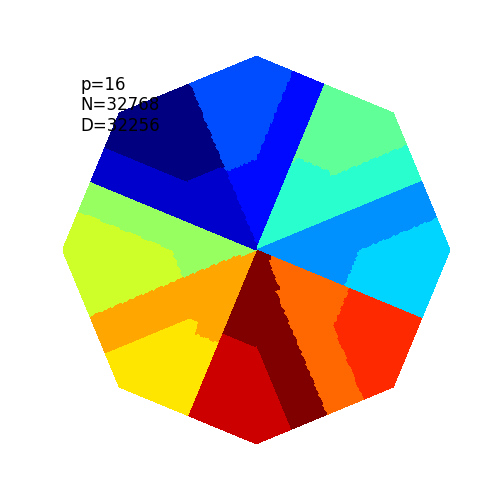
\includegraphics[width=0.45\linewidth]{poly8_6-16.png}
  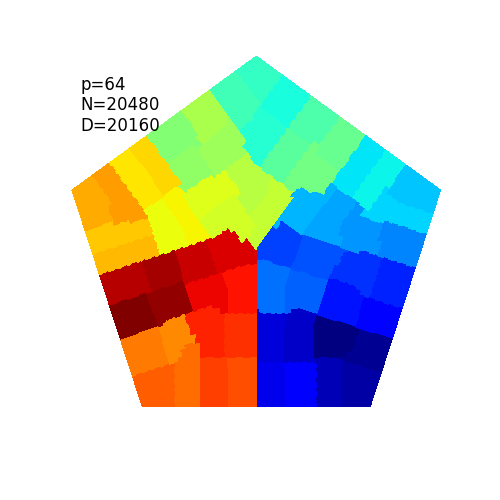
\includegraphics[width=0.45\linewidth]{poly5_6-64.png}
  \label{fig:mooi}
\end{figure}
\begin{figure}[h!]
	\center
  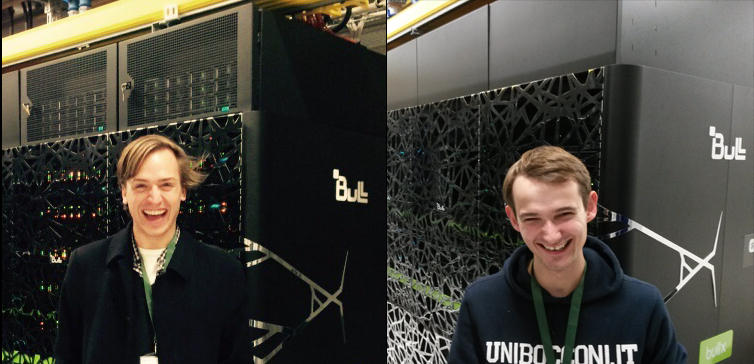
\includegraphics[width=\linewidth]{voorkantjuh.png}
   \caption*{Happy, because we're next to Cartesius}
\end{figure}
\vfill
  \end{center}
\end{titlepage}

\begin{abstract}
  In this report, we will be concerned with solving $Ax=b$ for \emph{spd} (symmetric positive-definite) $A$, with known $A$ and $b$. We will look at a parallel implementation of the Conjugate Gradient method, and apply this to sparse matrices in the sense that a lot of the elements are zero. This makes it possible to skip parts of the matrix-vector products one encounters. First, we will give our solution to Exercise~4.6 from \cite{biss04} by specifying a general-purpose parallel sparse CG implementation. We will improve on this to create a parallel sparse CG implementation for Finite Element matrices, given the extra knowledge that the matrix is not random, but has geometric meaning. We will conclude with a system of real-life size and compare the two methods.
\end{abstract}
%\maketitle
\tableofcontents
\hrulefill
\section{Introduction}
\begin{quote}
``The conjugate gradient method (CG) is an algorithm for the numerical solutions of particular systems of linear equations, namely those whose matrix is symmetric and positive definite. The conjugate gradient method is often implemented as an iterative algorithm, applicable to sparse systems that are too large to be handled by a direct implementation or other direct methods such as the Cholesky decomposition. Large sparse systems often arise when numerically solving partial differential equations or optimization problems." \cite{wiki:cg}
\end{quote}

\begin{quote}
``The finite element method (FEM) is a numerical technique for finding approximate solutions to boundary value problems for partial differential equations. It uses subdivision of a whole problem domain into simpler parts, called finite elements, and variational methods from the calculus of variations to solve the problem by minimizing an associated error function. Analogous to the idea that connecting many tiny straight lines can approximate a larger circle, FEM encompasses methods for connecting many simple element equations over many small subdomains, named finite elements, to approximate a more complex equation over a larger domain." \cite{wiki:fem}
\end{quote}

In this report, we will be concerned with solving $Ax=b$ for \emph{sspd} (sparse symmetric positive-definite) $A$, with known $A$ and $b$. We will use the Conjugate Gradient method as iterative solver. More specifically, we will be interested in parallelizing this method. 
In \S2--\S5, we will give our solution to Exercise~4.6 from \cite{biss04} by specifying a general-purpose parallel sparse CG implementation. We will test our implementation using random generated matrices.

In \S6 we will narrow our class of sspd matrices to matrices found in the Finite Element Method. These matrices have additional (geometrical) structure as they arise from solving a partial differential equation.  We will use this knowledge to create another parallel CG implementation specifically for FEM-matrices. These matrices occur reguarly in engineering and thus even have a practical use.

In \S7 we will test both our methods on a set of FEM-matrices. What method performs better? When does the CG method benefit from parallelizing, and how large does our system need to be?

We will provide thoughts for future work in \S10.

\section{CG}
In its most basic (sequential, non-preconditioned) form, CG can be written down as in Algorithm~\ref{alg:seqcg}. \cite[Alg.~4.8]{biss04} We slightly adapted it from its original form to be able to use the different BLAS \cite{blas} routines.

\begin{algorithm}[H]
\caption{Sequential CG}
\label{alg:seqcg}
\SetKw{KwStep}{step}
\SetKwInOut{Input}{Input}  
\SetKwInOut{Output}{Outout}
  \Input{$k_{max} \in \N$, $\e \in \R$, $n \in \N$, $A$ spd $n \times n$, $b \in \R^n$}
  \Output{$x \in \R^n$ with $Ax \approx b$}
   $k := 0$\;
   $u[n] = \vec 0, w[n]$\;
   $\rho_{old}, \beta$\;
  
   $r := b$\;
   $\rho := \langle r, r \rangle$\;
   $nbsq := \rho$\;
  
	 \While{$\rho > \e^2 \cdot nbsq \wedge k < k_{max}$} {
	\uIf{$k > 0$} {
       $\beta = \rho/\rho_{old}$\;
       $u \gets \beta u$\;\label{line:scaleu}
		}
    
     $u \gets r + u$\;\label{line:axpyu}
     $w \gets Au$\;\label{line:mvw}
     $\gamma := \langle u, w\rangle$\;\label{line:ipgamma}
     $\alpha := \rho/\gamma$\;
     $x \gets x + \alpha u$\;\label{line:axpyx}
     $r \gets r - \alpha w$\;\label{line:axpyr}
     $\rho_{old} = \rho$\;
     $\rho = \langle r, r \rangle$\;\label{line:iprho}
    
     $k = k+1$\;
	 }
\end{algorithm}

\subsection{Sparse CG}
As most real-life matrices are sparse in nature, we will adapt Algorithm~\ref{alg:seqcg} to a version that supports sparse matrices. We will assume the right-hand side to be dense. This allows us to effectively only change I/O and the function responsible for matrix-vector multiplication.

Our storage format uses the so-called coordinate scheme; we store tuples $(i, j, a_{ij})$ with $i$ the row number, $j$ the column number and $a_{ij}$ the matrix value at this position. The Matrix Market file format adds some headers, e.g. to denounce symmetry so that one only has to store the lower triangular part. We denote by $nz(A)$ the amount of nonzero elements in this lower triangular part. If we store the list of tuples in three lists of length $nz(A)$, namely $I$, $J$ and $v$, we can compute a sequential sparse matrix-vector multiplication using e.g.~\cite[Alg.~4.3]{biss04}.

\section{Parallellizing CG}
\label{sec:parcg}
With our sequential algorithm in hand, we are now ready to parallelize the Conjugate Gradient method. Given the spd matrix $A \in \R^{n \times n}$ and vector $b \in \R^n$, this requires us to find distributions for $A$, $b$ and all other vectors present in the algorithm. If we want to minimize communication cost, we desire that the distributions of $n, x, r, u, w$ are the same.\footnote{This was also pointed out in \cite[p.~174]{biss04}.} This allows us to perform all vector updates locally and makes for easy implementation of the inner product algorithm.

Every iteration of Algorithm~\ref{alg:seqcg} has 5 vector updates, two inner products and one matrix-vector multiplication. Finding good distributions of $A$, $x$ and $b$ is an NP-hard problem so we will have to resort to heuristic methods. To find these edistributions, we can use Mondriaan.\footnote{Mondriaan is a sequential program written in C that can be used to partition a rectangular sparse matrix, an input vector, and an output vector for parallel sparse matrix-vector multiplication. The program is based on a recursive bipartitioning algorithm that cuts the matrix horizontally and vertically, in a manner resembling some of the famous Mondriaan paintings. The algorithm is multilevel, hypergraph-based, and two-dimensional. It reduces the amount of communication and it spreads both computation and communication evenly over the processors. The program can partition hypergraphs with integer vertex weights and uniform hyperedge costs, but it is primarily intended as a matrix partitioner. \cite{mondriaan}} With its option \texttt{-SquareMatrix\_DistributeVectorsEqual=yes} we can force input and output vector to have the same distribution. We chose not to alter the default load imbalance option of $\epsilon = 0.03$.\footnote{Later inspection using the formula provided in \cite[p.~189]{biss04} -- $\epsilon = Vg/(2nz(A))$ being optimal for the matrix-vector product -- revealed that the optimal value (which of course depends on $p$ and $A$) lies around $0.2$. The total iteration time was however not that much faster, so we opted not to rerun everything.}

The resulting parallel algorithm is in appearance almost exactly as Algorithm~\ref{alg:seqcg}, so we will not rewrite this. As the vector updates can be done locally without communication, BLAS routines were used (just as in the sequential algorithm). The big changes are made in computation of the inner product and the matrix-vector product. The \texttt{bspmv} algorithm found in \cite[Alg.~4.5]{biss04} was used without alterations, but the \texttt{bspip} algorithm \cite[Alg.~1.1]{biss04} was found unusable as this assumed a cyclical distribution. See Algorithm~\ref{alg:ip} for a parallel inner product algorithm that only assumes that both vectors have the same distribution. The beauty of this algorithm is that no processor has to know the distribution, as long as it has its own vector components stored as a smaller vector.

\begin{algorithm}
  \caption{Parallel inner product $\langle v, y \rangle$ assuming $v$ and $y$ have equal distributions}
  \label{alg:ip}
	\SetKw{KwStep}{step}
	\SetKwInOut{Input}{Input}  
	\SetKwInOut{Output}{Outout}
    \Input{$p$ total number of processors, $0 \leq s < p$ current processor number, $nv_s$ the amount of vector elements locally stored, $v_s,y_s \in \R^{nv_s}$ local vectors}
    \Output{$\alpha = \langle v, y \rangle$}
		$\alpha_s := 0$\;
		$\alpha := 0$\;
		\tcc{Compute local inner product}
		\For{$i = 0$ to $nv_s$} {
			$\alpha \gets \alpha + v_s[i] \cdot y_s[i]$
		}
		\tcc{Put local inner prodcut}
		\For{$q = 0$ to $p$} {
			Put $\alpha_s$ to $P(q)$\;
		}
		\tcc{Find global inner product}
		\For{$q = 0$ to $p$} {
			$\alpha \gets \alpha + \alpha_q$\;
		}
\end{algorithm}

\subsection{BSP cost}
We first calculate the BSP cost of the parallel algorithm per iteration, using Algorithm~\ref{alg:seqcg} as reference. Let $nv_s$ be the amount of vector elements locally stored on processor $s$. The rescale costs $nv_s$ operations and \texttt{axpy}s cost $2nv_s$ each. This makes vector updates contribute $7nv_s$ to the total amount of operations. 

Looking at Algorithm~\ref{alg:ip}, each inner product yields $2nv_s - 1$ operations for Superstep 1, $pg$ operations for Superstep 2 and $p-1$ operations for Superstep 3, with 2 synchronizations in between for a total of $2(2nv_s - 1 + p-1 + pg + 2l)$ inner product operations per iteration.

We found in \cite[p.~189]{biss04} that the matrix-vector product using a Mondriaan distribution yields a total BSP cost of $2(1+\epsilon)nz(A)/p + Vg/p + 4l$ operations. We have one such matrix-vector product per iteration.

Summing everything together, we get a total BSP cost per iteration of
\[
  11nv_s - 4 + p(2+2g) + (Vg + 2 (1+\epsilon)nz(A))/p + 8l.
\]

We were unable to further specify this without getting into very nasty details.

\section{Cartesius hardware}
\label{sec:cart}
We ran \texttt{bspbench} with the default $n=100$, $h=256$ and $p \in \{1, \ldots, 64\}$ to get an idea of values for $r$, $g$ and $l$ for processor counts and get an idea of the scaling properties of Cartesius.

We found the average value of $\bar r = 9157$ Mflop/s. See Figure~\ref{fig:cart} for values of $g$ and $l$ as function of $p$. We see a sharp increase in both $g$ and $l$ at $p=24$. These have to do with the hardware of Cartesius: under 24 cores is done on a shared-memory system, where communication is cheap.

\begin{figure}
  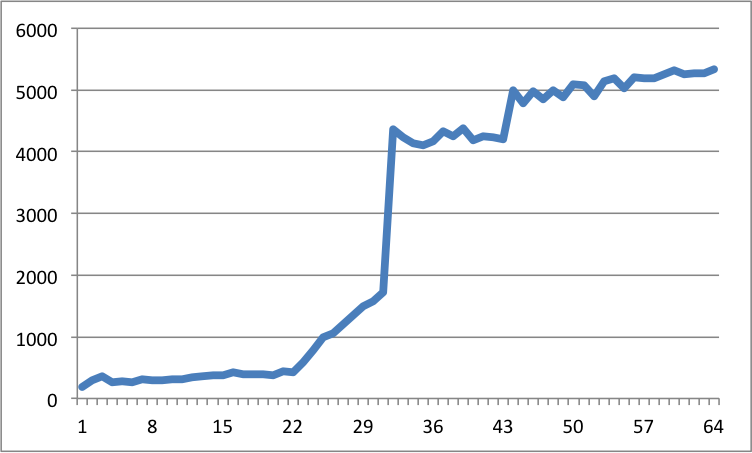
\includegraphics[width=0.49\linewidth]{cartg.png}
  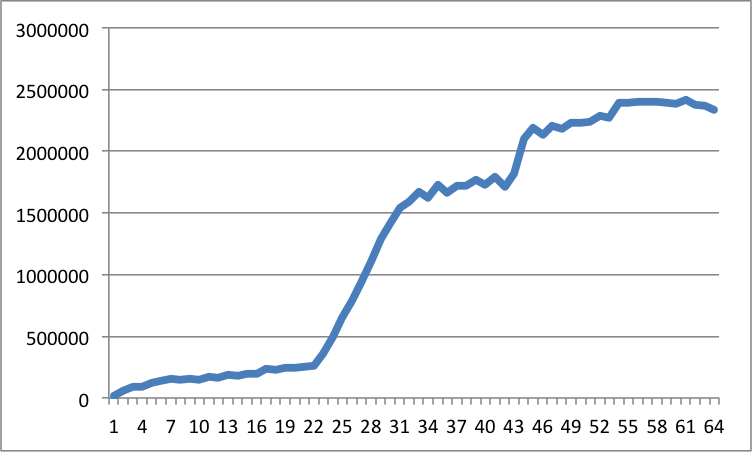
\includegraphics[width=0.49\linewidth]{cartl.png}
  \caption{Results of running \texttt{bsbench} on a thin node of Cartesius with $n=100$, $h=256$. $x$-axis: $p \in \{1, \ldots, 64\}$. $y$-axis: left -- $g$, right -- $l$.}
  \label{fig:cart}
\end{figure}

\section{Testing our parallel CG}
To test our implementation, we want to have access to a lot of similar matrices. One way to do this is described in \cite[Ex.~4.6]{biss04}: create a random sparse matrix $B$ with values in $[-1,1]$, then take $A \gets B + B^\top + \mu I$ with $\mu$ such that $A$ is strictly diagonally dominant. As the idea of this is merely to generate a matrix $A$ that is spd, we opted for a slightly easier approach. 

We need to compute a \emph{symmetric} matrix, so we only have to look at the lower triangular part of this matrix. First we create a random sparse strictly lower triangular matrix $B$. We do this by specifying some density $\delta$ and placing a random number in $[-1,1]$ on position $(i,j)$ with probability $\delta$. The matrix must be positive definite, which is achieved \cite[Ex.~24.2]{trefbau} if
\[
  |A_{ii}| > \sum_{j=1, j\ne i}^n |A_{ij}|= \sum_{j=1}^{i-1} (|B_{ij}| + |B_{ji}|).
\]
Let $\mu$ be the maximum of the row sums. We now know that $B + B^\top + \mu I$ is an spd matrix. Finally, to add some more randomness to the diagonal, we replace the diagonal element $\mu$ by a random number in $[\mu, \mu + 2]$ with probability $\delta$.

This method, and its counterpart given in \cite[Ex.~4.6]{biss04}, has one glaring drawback. Matrices of this type are diagonally dominant, implying that the diagonal elements are \emph{much} larger than the offdiagonals! The resulting matrix is close to diagonal. As solving $Ax=b$ for diagonal $A$ using CG completes in one step, it will be no surprise that every test with matrices like these will result in very few iterations.

We created a lot of systems,\footnote{We varied $n$ between $2^6$ and $2^{12}$, $\delta := nz(A)/n^2$ between $0.01$ and $0.2$ with 6 values and $p$ between $2^0$ and $2^6$ for a total of about 300 matrices. } and for each system computed:
\begin{gather*} 
P, n, nz(A), \delta = nz(A)/n^2, k \text{(number of iterations)}, \\
t_i~ \text{(time to initialize)}, \quad t_{mv}~ \text{(time matrix-vector)}, \quad t_{ip}~ \text{(time inner product)}, \\
t_l~ \text{(time local operations)}, \quad t_g~ \text{(time spent computing global solution)}, \\
t_c = t_{mv} + t_{ip} + t_l~ \text{(time spent in while-loop)}, \quad t = t_i + t_{mv} + t_{ip} + t_l + t_g~ \text{(total time)}.
\end{gather*}

We did a lot of testing and came to the conclusion that $k\sim 10$ -- being the order of amount of iterations needed for CG to converge --  is too low to get any significant result, as communication time is just too much of a contribution. 

We varied the right-hand side by either (1) setting $b := \vec 1$ (simple right-hand side), (2) $b := A\vec 1$ (known solution), (3) $b_i \in [0, 1]$ (random right-hand side) and (4) the ability to load $b$ from file. The last method proved very useful later on, when comparing this algorithm with our special-purpose FEM-CG. One conclusion of some significance is that the iteration count (and the total time) is more or less invariant under the choice of right-hand side.

\subsection{Example}
Taking $n = 4096$ and $\delta \in \{0.1, 0.2\}$, we get two sample matrices. Looking at $t_{mv}$ and $t_{ip}$ for these matrices yields Figure~\ref{fig:samples}. We see that the computation time ($t_c = t_l + t_{mv} + t_{ip} \approx t_{mv} + t_{ip}$ for small systems with little computations) decreases first, then increases later. This has to do with the Cartesius hardware: see \S \ref{sec:cart}.

If we look at $t_{ip}$ separately, one sees that $t_{ip}$ takes the overhand, especially in the non-shared memory case. The systems are simply too small for parallelization to be of use; the time spent computing the local inner product is heavily outweighed by the communication costs. This raises the question if $t_{ip}$ would improve had we used the inner product communication strategy from the first homework exercise. \cite{TODOHUISWERK} In this exercise, we found that if
\[
  (p - 5\log_2 p) + (p + \log_2 p - 1)g + (2-\log_2 p)l > 0
\]
the new strategy is better. A quick inspection yields that this is true for $p \leq 4$ and \emph{very} false (values being in the order of negative millions) for $p > 4$, so we didn't even try.

\begin{figure}
  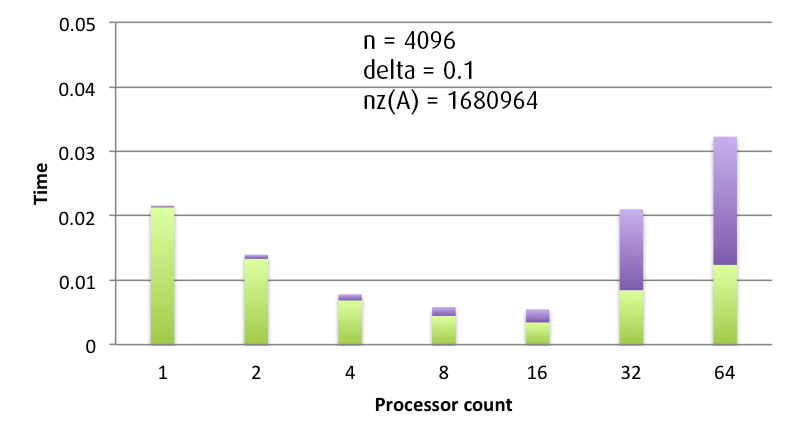
\includegraphics[width=0.48\linewidth]{n4096d0_1mvip.png}
  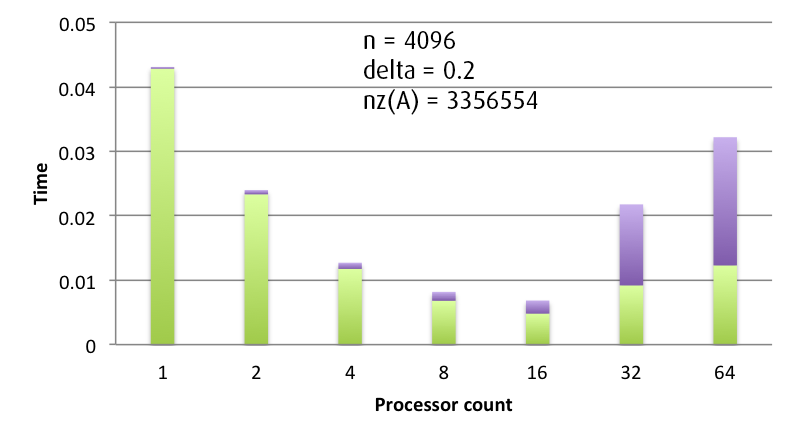
\includegraphics[width=0.48\linewidth]{n4096d0_2mvip.png}
  \caption{Timing results for two sample matrices. Purple: $t_{ip}$; green: $t_{mv}$.}
  \label{fig:samples}
\end{figure}


\section{FEM and CG}
We are now trying to solve a FEM system using CG. More specifically, we want to find a (numerical) solution to the two-dimensional PDE
\begin{equation}
  \label{eqn:fem}
  \begin{cases} -\Delta u = f & \text{ in } \Omega \\ u = 0 & \text{ on } \partial \Omega \end{cases}
\end{equation}
with $\Omega$ a polygonal domain. In this report, we will look at $f=1$, further narrowing the problem.

The idea of the Finite Element Method is to find the projection of $u \in C^2_0(\Omega)$ -- twice continuously differentiable functions that are zero on the boundary of $\Omega$ -- onto some (finite dimensional) linear subspace $V$. We will take $V$ to be the space of piecewise linear functions, subject to some partitioning of $\Omega$ into \emph{elements}. Often, these elements will be triangular (and hence, we will use triangles and elements interchangeably from here on after). Choosing $\Omega$ to be polygonal allows us to triangulate $\Omega$ into triangles $T = \{ T_0, \ldots T_{N-1}\}$ such that $\Omega = \cup_{k = 0}^{N-1}T_k$. We will denote the vertices of these triangles with $X = \{x_0, \ldots, x_{n-1}\}$ and order them such that $x_0, \ldots, x_{D-1}$ lie in $\Omega$ with $x_{D}, \ldots, x_{n-1}$ on $\partial \Omega$.

This triangulation cannot be arbitrary, as this introduces \emph{hanging nodes} and other nasty side-effects. We assume triangulations to be \emph{conforming}; in this report, this means that ``everything works nicely''.

The fact that functions in $V$ are zero on the boundary implies that $\dim(V) = D$. The number $D$ is also called the \emph{degrees of freedom} for a given triangulation. A useful basis for this subspace $V$ is the \emph{nodal} basis $\Phi = \{\phi_i: 0 \leq i < D\}$ of hat functions, uniquely determined by the property
\[
  \phi_i( x_j) = \delta_{ij} \quad \forall~~0 \leq i < D,\, 0 \leq j < N.
\] An example of such a basis function is given in Figure~\ref{fig:nodal}. Note that every basis function $\phi_i$ directly corresponds to a vertex not lying on the boundary. This allows us to identify vertices with basis functis: every degree of freedom is coupled to a vertex inside the domain.
\begin{figure}[h!]
	\centering
	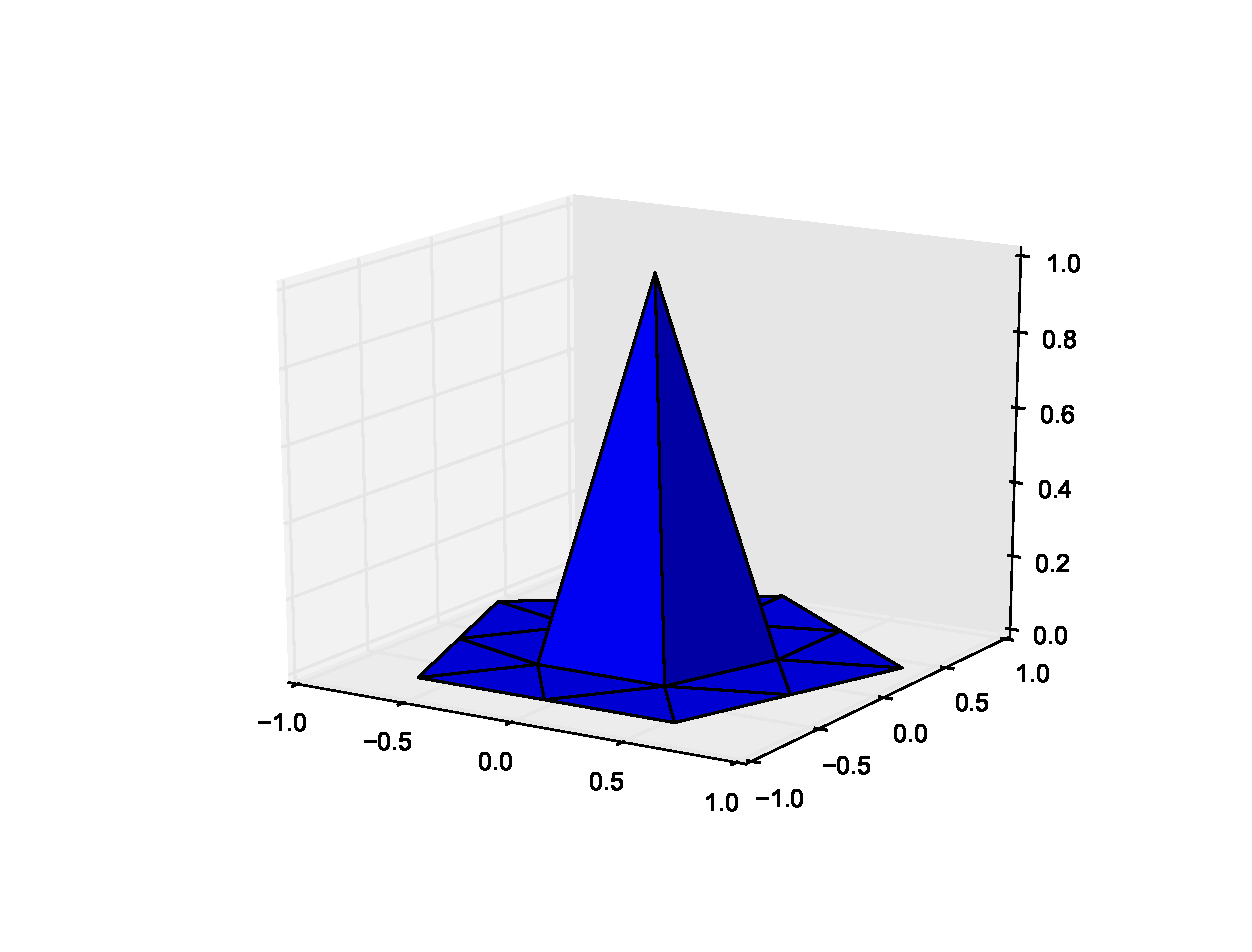
\includegraphics[width=0.5\linewidth]{nodal_vijfhoek.eps}
\caption{Example of a basis function for a pentagon}
\label{fig:nodal}
\end{figure}

The crux of the Finite Element method is that we can actually find the projection $u_V$ of $u$ onto $V$ \emph{without knowing the exact solution $u$}! Write $u_V$ in the nodal basis:
\[
  u_V = \sum_{i=0}^{D-1} \alpha_i \phi_i.
\]
Then, $u_V$ can be proven \cite{TODO} to be the solution to the system
\[
	A\vec \alpha = b \text{ with }  A_{ij} := a(\phi_i, \phi_j) = \int_\Omega \nabla \phi_i \cdot \nabla \phi_j \text{ and } b_i = \int_\Omega \phi_i.
\]

The matrix $A$ is called the \emph{stiffness matrix}, which is spd.\cite{TODORAYMOND} It is also a sparse matrix, as the basis functions only `interact' with a small number of neighbours.

In the coming sections, we will look at the two steps involved in solving such a FEM-system:
\begin{description}
  \item[System assembly] is the act of finding the nonzeros of $A$ and $b$;
  \item[Solving the system] as $n$ (and thus $D$) is generally very large, we want to use an efficient solver. We will be using CG.
\end{description}

\subsection{System assembly}
How can we find the elements of the stiffness matrix in an efficient manner? In other words, how do we calculate $a(\phi_i, \phi_j)$? The following elegant derivation uses the fact that the domain can be decomposed into triangles:
\begin{equation}
  \label{eqn:div}
	a(\phi_i, \phi_j) = \int_\Omega \nabla \phi_i \cdot \nabla \phi_j = \int_{T_0 \cup \dots \cup T_{N-1}} \nabla \phi_i \cdot \nabla \phi_j = \sum_{n = 0}^{N-1} \int_{T_n} \nabla \phi_i \cdot \nabla \phi_j =: \sum_{n=0}^{N-1}a_{T_n}(\phi_i, \phi_j).
\end{equation}

We will call the matrix $A_T$ with $(A_T)_{ij} = a_T(\phi_i, \phi_j)$ the \emph{element matrix} of triangle $T$, which contains information on interactions of basis functions restricted to $T$. This reduces the problem of finding the stiffness matrix to finding the element matrices. Note that these matrices are very sparse: in fact, they only have $3 \times 3$ nonzeros as there are only 3 basis functions that have interactions per triangle. Therefore, we will compute a $3 \times 3$ matrix $\hat A_T$ and scale this up to the $D \times D$ element matrix $A_T$.


In fact, this $3 \times 3$ matrix can be computed in a variety of ways. One way is to use
\[
  D = \begin{bmatrix} v_{0} & v_{1} & v_{2} \end{bmatrix} \in \R^{ 2 \times 3}
\]
with $v_{i}$ the $i$th vertex of triangle $T$. Then one can prove \cite{TODO} that
\[
  \hat A_T = \frac{D^\top D}{4 \cdot \text{vol}(T)}
\]
with $\text{vol}(T)$ the volume of triangle $T$.

We can compute the right-hand side $b_i$ in much the same way. One can prove \cite{TODOjan} that
\[
  b_i = \int_\Omega \phi_i = \sum_{n=0}^N \int_{T_n} \phi_i
	= \sum_{n=0}^N \mathbf{1}_{T_n}(x_i)\text{vol}(T_n)/3.
\]

With these notes we can easily derive Algorithm~\ref{alg:calc_fem} which constructs a FEM-system for a given triangulation.

\begin{algorithm}[H]
\SetKw{KwStep}{step}
\SetKwInOut{Input}{Input}  
\SetKwInOut{Output}{Outout}
\Input{$X : $ list of vertices, \\
       $T : $ list of $N$ triangles, \\
		   $D : $  degrees of freedom.}
\Output{$ A : $ sparse $d\times d$ FEM-matrix , \\
	      $ b : $ vector of length $D$, the rhs of the system.}
	\tcc{Initalize to zero}
	$b := 0$\;
	$A := 0$\;
	\For{$k : 0 \leq k < N$} {
		Generate element matrix $\hat A_{T_k}$\;
		\tcc{Loop over indices in the element matrix}
		\For{$li : 0\leq li < 3$} {
			Calculate global index $i$ corresponding to $li$\;
			\tcc{Check if vertex $li$ corresponds to a DOF}
			\uIf{$i < D$} {
				$b_i = b_i + \text{vol}(T_k)/3$\;
				\For{$lj : 0 \leq lj < 3$} {
					Calculate global index $j$ corresponding to $lj$\;
					\uIf{$ j < D$} {
						$A_{i,j} := A_{i,j} + (A_{T_k})_{li,lj}$\;
					}
				}
			}
		}
	}
 \caption{Calculate the FEM-matrix.}
 \label{alg:calc_fem}
\end{algorithm}
\subsection{Solving the system}
In the previous section we saw how to assemble the FEM system. One could use this approach to create a `naive' parallel FEM solver: let one processor assemble the system, find a parallel distribution (using e.g. Mondriaan) and apply the parallel CG algorithm described in \S\ref{sec:parcg}. This has a few disadvantages:
\begin{enumerate}
  \item[(I)] Matrix assembly is computationally expensive;
  \item[(II)] This system is possibly enormous, limiting us to systems that fit in memory of a single processor;
  \item[(III)] The relation between the geometrical object, triangulation and nonzeros is lost: $a_{ij}$ is nonzero iff $\phi_i$ and $\phi_j$ interact, which only happens if $x_i$ and $x_j$ are connected by an edge.
\end{enumerate}

We will look at a smarter approach which solves these disadvantages. Instead of distributing the matrix nonzeros $A_{ij}$ between processors, we distribute the triangles $T_n$ over $p$ processors, thereby solving disadvantage (III). We divide our triangulation into $p$ disjoint sets of length $N_q$
\[
  T = \bigsqcup_{q=0}^{p-1} T^q, \quad T^q = \{ T^q_0, \ldots, T^q_{N_q-1} \},
\]
leading to the partition $\Omega = T^0 \cup \dots \cup T^{p-1}$. When distributing the triangles over the processors, we implicitly distribute the vertices over the processors as well.  A side-effect of this is that a vertex $x_i$ can belong to multiple processors. Therefore we define its \emph{processor set} 
\[
  \Pi: \{0, \ldots, D-1\} \to 2^{\{0, \ldots, p-1\}}: i \mapsto \Pi(i)
\]
as the set of processors that contain $x_i$ in one of their triangles. Remember that every vertex was identified with a degree of freedom. As vertices might be shared with different processors, this induces a different kind of vector distrbution than the one described in \cite{biss04}: all the processors in a set must have a copy of the corresponding vector value.
Figure~\ref{fig:procset} is an illustration of the definitions given in the previous section. 

\begin{figure}[h!]
  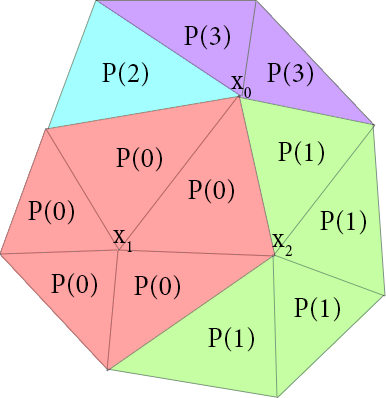
\includegraphics[width=0.5\linewidth]{procset.png}
  \caption{A sample mesh with its triangle distribution. Only vertices not on the boundary have been numbered. For these vertices, $\Pi(0) = \{0, 1, 2, 3\}, \Pi(1) = \{0\}, \Pi(2) = \{0, 1\}$.}
  \label{fig:procset}
\end{figure}
\subsection{Matrix-vector calculation}
To implement CG with our new distribution we need to calculate the matrix-vector $u = Av$. This is where we profit from using the geometrical relation between the triangle distribution and the stiffness matrix $A$. Use of equation \eqref{eqn:div} leads to a natural decomposition of $A$ into
\[
	A = \sum_{q=0}^{p-1} A^q\quad \text{ with } A^q= \sum_{n=0}^{N_q-1} A_{T^q_n} \quad \text{ and } (A^q)_{ij} = \sum_{n=0}^{N_q-1} a_{T_n}(\phi_i,\phi_j).
\]
The matrices $A^q$ are $D \times D$ but again very sparse. We identify $A^q$ with a smaller matrix $\hat A^q$ by removing zero rows and columns. As the name suggest, the processor $q$ constructs the matrix $A^q$ (actually $\hat A^q$) locally. This is possible because $A^q$ only depends on triangles that are distributed to processor $q$.

To calculate the entire product $u = Av$, we will first calculate $v^q = A^q u$ (actually $\hat v^q = \hat A^q \hat u$). We can find $v$ by adding these local vectors: $v = \sum_{q =0}^{p-1} v^q$. Remember that vector element $v_i$ corresponds to a vertex $x_i$, which is shared by the processors in the set $\Pi(i)$. We calculate the value $v_i$ by letting every processor in the set $\Pi(i)$ send $(v^q)_i$ to every other processor in $\Pi(i)$. After this communication step, every processor sums over these local values to find $v_i$. This method ensures that every processor sharing vertex $x_i$ gets the correct value of $v_i$. In Algorithm~\ref{alg:fem_mv} we give the implementation of the parallel $u = Av$ for a FEM-matrix $A$.

\begin{algorithm}[H]
\SetKw{KwStep}{step}
\SetKwInOut{Input}{Input}  
\Input{$A^s: $ sparse (local) FEM-matrix for $P(s)$, such that
	     $A = \sum_{t=0}^{p-1} A^t$, \\
       $\Pi : \{0, \dots, D-1\} \to 2^p$, \\
			 $v : $ vector of length $D$, $\text{distr}(v) = \Pi$.}
\KwOut{$u : Av$, $\text{distr}(u) = \Pi$}
	\nlset{(0)}
	Local sparse symmetrical matrix-vector $u_s = A^s v$ by $\hat u_s = \hat A^s \hat v$\;
	\nlset{(1)}
	\For{$ i : 0 \leq i < D \wedge s \in \Pi(i)$} {
		\For{$t \in \Pi(i)$} {
			put $(u_s)_i$ in $P(t)$\;
		}
	}
  
  \nlset{(2)}
	\For{$ i : 0 \leq i < D \wedge s \in \Pi(i)$} {
		$u_i := 0$\;
		\For{$t \in \Pi(i)$} {
			$u_i := u_i + (u_t)_i$\;
		}
	}
 \caption{Matrix-vector product for a FEM-system for $P(s)$}
 \label{alg:fem_mv}
\end{algorithm}

\subsection{Creating $\hat A^q$}
To create $\hat A^q$, we need to identify the zero rows (and by symmetry, columns) of $A^q$. A row $i$ is zero if $(A^q)_{ij} = 0$ for $0 \leq j < D$; this corresponds to the situation where basis function $\phi_i$ has no interactions on any of the triangles contained by processor $q$.  Translating this back to the triangulation, we see that this happens if processor $q$ does not use vertex $x_i$: $q \not \in \Pi(i)$. This gives us an explicit formula for $D_q$, defined as the size of $\hat A^q$:
\[
	D_q = \#\{ i : 0 \leq i < D,\, q \in \Pi(i)\}.
\]

Algorithm~\ref{alg:init_fem} now describes how to create $\hat A^q$ for each processor, given a distribution $\psi$ of the triangles. Here  we assume that the initial distribution is entirely read by processor $0$.


\begin{algorithm}[H]
\SetKw{KwStep}{step}
\SetKwInOut{Input}{Input}  
\SetKwInOut{Output}{Outout}
\Input{$X :$ list of $n$ vertices, with first $D$ vertices corresponding to a DOF, \\
	     $T : $ list of $N$ triangles, $\text{distr}(T) = \psi$.}
\Output{$\Pi:$ processor set for each DOF, \\
	     $\Pi_{\text{owner}}:$ the `owner' of a DOF, \\
			 $\hat A^s: $ local sparse FEM-matrix for $P(s)$, \\
			 $b : $ vector of length $D$, $\text{distr}(b) = \Pi$.}
  \nlset{(0)}
	\If{$ s = 0$} {
		Use $\phi$ to calculate $\Pi$, the processor set for each DOF\; 
		Put the local amount of DOF, vertices and triangles in each processor\;
	}
  \nlset{(1)}
	Allocate memory for the (local) FEM data\;
	\nlset{(2)}
	\If{$ s= 0$} {
		\For{$i : 0 \leq i < N$} {
			put $T(i)$ in $P(\psi(i))$\;
			put vertices of $T(i)$ in $P(\psi(i))$ \tcc*[h]{Avoid duplicates in implementation}
		}
	}
  \nlset{(3)}
	Calculate local FEM-matrix $\hat A^s$ and local right hand side $\hat b^s$\;
	
  { Produce the entire vector $b$, same method as described in Alg~\ref{alg:mv_fem} }
	\nlset{(4)}
	Communicate entries of $\hat b^s$ to processor sets, see superstep $(1)$ in Alg~\ref{alg:mv_fem}\;
	\nlset{(5)}
	Sum the values to find $b$, see superstep $(2)$ in Alg~\ref{alg:mv_fem}\;
 \caption{Algorithm that calculates the local FEM data.}
 \label{alg:init_fem}
\end{algorithm}

\subsection{Inner product}
The CG Algorithm also requires the inner product between two vectors. We calculate this inner product using a slightly altered version of Algorithm~\ref{alg:ip}. In the new case, the vector elements are duplicated on every processor in the corresponding processor set. Therefore, for each vector element we must make a choice which processor from the processor set adds the contributions of this element to the inner product. We define this choice by the creating an operator that gives an `owner' of each vector element:
\[
	\Pi_{\text{owner}}(i) \in \Pi(i).
\]

In our implementation we chose to make the processor with the lowest number the owner; $\Pi_{owner}(i) := \min \Pi(i)$. The parallel inner product algorithm for these distributions is now given in Algorithm~\ref{alg:fem_ip}.


\begin{algorithm}[H]
\SetKw{KwStep}{step}
\SetKwInOut{Input}{Input}  
\Input{$x,y : $ vector of length $D$, \\
	     $\Pi_{\text{owner}} : \{0, \dots, D-1\} \to P$,\\
			 $\text{distr}(x) = \text{distr}(y) = \Pi_{\text{owner}}.$}
\KwOut{$a  := \langle x, y\rangle$}
\nlset{(0)}
  $a_s := 0$\;
	\For{$ i: 0 \leq i < D \wedge \Pi_{\text{owner}}(i) = s$} {
	  $a_s := a_s + x_i y_i$\;
	}
\nlset{(1)}
  \For{$ t: 0 \leq t < p$} {
		put $a_s$ in $P(t)$\;
	}
\nlset{(2)}
  $a := 0$\;
  \For{$ t: 0 \leq t < p$} {
		$a := a + a_t$\;
	}
 \caption{Inner product for vectors in FEM-system for $P(s)$}
 \label{alg:fem_ip}
\end{algorithm}

\subsection{CG on FEM-system}
In the previous sections, we have given a way to calculate the matrix-vector and inner product for a FEM system, defined by a mesh and a triangle distribution, contrasting to an actual distribution of the stiffness matrix nonzeros, which we used in \S\ref{sec:parcg}.

With both these operators the implementation of CG is similar to the sequential one described in Algorithm~\ref{alg:seqcg}; we just have to replace the inner product and matrix-vector product with the algorithms described above.
\subsection{Triangle distribution}
The triangle distribution $\psi$ determines the cost of the operations described above. For a vertex $x_i$, there are two possibilities:
\begin{enumerate}
  \item $|\Pi(i)| = 1$. This means that all interactions of the basis function $\phi_i$ are stored on a single processor $q$, meaning that $(Av)_i = (A^qv)_i$ or in other words, no communication is necessary. This corresponds with $x_0$ in Figure~\ref{fig:procset};
  \item $|\Pi(i)| > 1$. Interactions of $\phi_i$ are stored on different processors. To compute $(Av)_i$, we need to communicate with $|\Pi(i)|-1$ processors. This corresponds with vertices $x_1, x_2$ in Figure~\ref{fig:procset}.
\end{enumerate}

Here we see another advantage of our FEM-approach. By distributing triangles, we can balance computation and communication cost of a matrix-vector multiplication. We chose to use Mondriaan, using \cite{bissmondriaan,biss2012}. We transform a given triangulation into a \emph{hypergraph} $H = (V,E)$ -- a generalization of a graph in which any number of hypervertices can be connected by hyperedges or \emph{nets}. This is done as follows:
\begin{itemize}
  \item[-] Every triangle $T_n$ in our triangulation is identified with a hypervertex $v_n \in V$;
	\item[-] Every vertex $x_i$ connecting triangles $\{T_{n_0}, \ldots, T_{n_k}\}$ is identified with a net (hyperedge) $e_i \in E$ connecting hypervertices $\{v_{n_0}, \ldots, v_{n_k}\}$.
  \item[-] Every hypervertex $v_n \in V$ is given a \emph{vertex weight}, measuring the computational cost corresponding with triangle $T_n$. In our case, one needs to compute the same quantities for every triangle.\footnote{In more advanced Finite Element methods where the polynomial degree is different for each triangle, this would scale with the polynomial degree.} We set this to 1;
  \item[-] Every net $e_i\in V$ is given a \emph{net weight}. Mondriaan does not implement this, but to be future-proof, we set this to 1 for all vertices $v_i$ not on the boundary and 0 for boundary vertices. This reflects the fact that boundary vertices have no degree of freedom attached to it and thus add no cost to the FEM-system.
\end{itemize}
Mondriaan will then find a partitioning of the vertices over the processors, such that the total communication volume is minimized while balancing the computation cost. Remember that vertices in the hypergraph correspond to triangles in triangulation. This implies that Mondriaan gives us a triangle distribution with the following properties:
\begin{align*}
  \text{Communication Volume}&= \sum_{i=0}^{D-1} |\Pi(i)| (|\Pi(i)| -1 ) \text{ is minimal for}\\
	|T^q| & \leq (1 + \epsilon) \frac{|T|}{p} \quad 0 \leq q < p.
\end{align*}

One intuitively sees that this minimizes the total communication while balancing the computation cost of the matrix-vector product. Unfortunately we were not able to derive an explicit BSP cost estimation for our algorithm, as the amount of triangles per processor is not directly related to the amount of computation needed in the processing step. We are not entirely sure whether the distribution Mondriaan creates actually satisfies these constraints as it lacks some features in hypergraph partitioning (such as net weights as described above). One could resolve this by using a different partitioner; see \S\ref{sec:future}.

In our implementations we chose $\epsilon = 0.1$, as this seems to generate reasonable distributions. An example of a distributions is given by the cover image. This represents the triangle distribution of a triangulation for the  regular 8- and 5-polygon. The different colors indicate parts of the triangulation that are owned by different processors. The triangulation on the left is divided among 16 processors, the right one among 64 processors. 
\subsection{Implementation details}
The algorithms presented so far as mostly given in pseudo-code. Here we want to hightlight a few implementation details that might be oversimplyfied in pseudo-code.
\subsubsection*{FEM Matrix}
Algorithm~\ref{alg:calc_fem} gives way to assemble the stiffness matrix. Here
we assumed to have a method for inserting or adding nonzeros at arbritary positions in the matrix. However,
this is not easily done in most data structures for sparse matrices as we do not know the
indices holding a nonzero beforehand. We adapt the following strategy: we first create a list
of all the nonzeros to add together in the coordinate scheme $(i,j,a_{ij})$.
This list will contain multiple elements with the same index $i,j$ when
the basis function $i$ and $j$ interact on multiple triangles. Afterwards, we know
exactly what indices contain a nonzero. We then convert this triple format to the \emph{ICRS}
\cite[p.~171]{biss04} format, after which we remove the duplicate nonzero entries by summing their values.

As the matrix is symmetric we only store the lower triangular part. In Algorithm~\ref{alg:fem_mv}
we calculate the matrix-vector product of the stiffness matrix and a vector. Algorithms for this
follow easily from the ICRS data structure. We implemented this like \cite[Alg.~4.4]{biss04}, with
a slight alteration to use symmetry.

\subsubsection*{Indexing}
In Alg~\ref{alg:fem_mv} we have to communicate values corresponding to a shared vertex. Here we have an indexing problem, as each (shared) processor has a different local index for the vertex. We solve this by using the orginal, or \emph{global} index. This is the index of the vertex in the initial triangulation. Each processor uses \verb=mpi_send= with the global index as tag to send the value to the other processors. Furthermore, each processor gets an array \verb=global2local= in the init stage that converts a global vertex index to a local one.


In superstep (1) of Algorithm~\ref{alg:fem_mv}, we do not have to communicate $(u^s)_i$ values if $\Pi(i) = \{s\}$. To do this efficiently we have chosen to first store the shared vertices and then stored the vertices for which we have $\Pi(i)=\{s\}$. As processor $s$ is the only processor we do not need to store the entire processor set for this vertex.

\section{Testing the new algorithm: Numerical results}
Initially, we had created a very large set with test triangulations to run our implementation on.\footnote{\emph{From the original report.} We chose to run our implementation on a few regular polygons with sides $k \in \{3, \ldots, 8\}$, creating initial triangulations with $k$ triangles (put a vertex in the middle and connect each edge with this vertex to create a triangle). We then made $n$ uniform refinements for $n \in \{1, \ldots, 7\}$, each time quadrupling the amount of triangles in the triangulation. This yielded a vast amount of test data with $D$ between 6 and 48768. On each of these triangulations, we used $p \in \{1, 2, 4, \ldots, 64\}$.} After our session on the second to last day, Raymond went home to fix some existing bugs in the code, enabling us to scale up even bigger. The final test run is therefore not on a large amount of small systems, but rather on one system of real-life proportions.

To compare our new algorithm with the original parallel CG implementation, we further created a script that creates the stiffness matrix and right-hand side, and writes them to file. As our original implementation allows for loading right-hand sides from file, we were able to plug-and-play. See the cover for a few examples.

Firstly, we see that Mondriaan does a tremendous job balancing the triangle distribution. Another thing we see is that we achieved speedup in all cases. Moreover, $t_{mv}$ is drastically improved. Inner product time is more or less the same, and initialization time is (somewhat surprisingly) improved as well.

First, we will look at the total iteration time as a function of $n$ (number of refinements), for different processor counts. See Figure~\ref{fig:times}. We see that for small systems ($n < 5$), parallelization is of no use. There is a distinct moment where parallelization on a shared-memory systems starts to make sense -- between $n=5$ and $n=6$. This is the moment where computation time is sufficient to computer the overhead of communication. For non-shared memory systems, this moment is less defined but still visible, as $p \in \{32,64\}$ are tied with sequential around $n=7$, but come out ahead from there. We see that starting from $n=10$, $p=64$ is actually faster than $p=16$, indicating that non-shared wins over shared-memory systems from here. The beauty is that these points actually hold for both the FEM algorithm and the CG algorithm.
\begin{figure}
  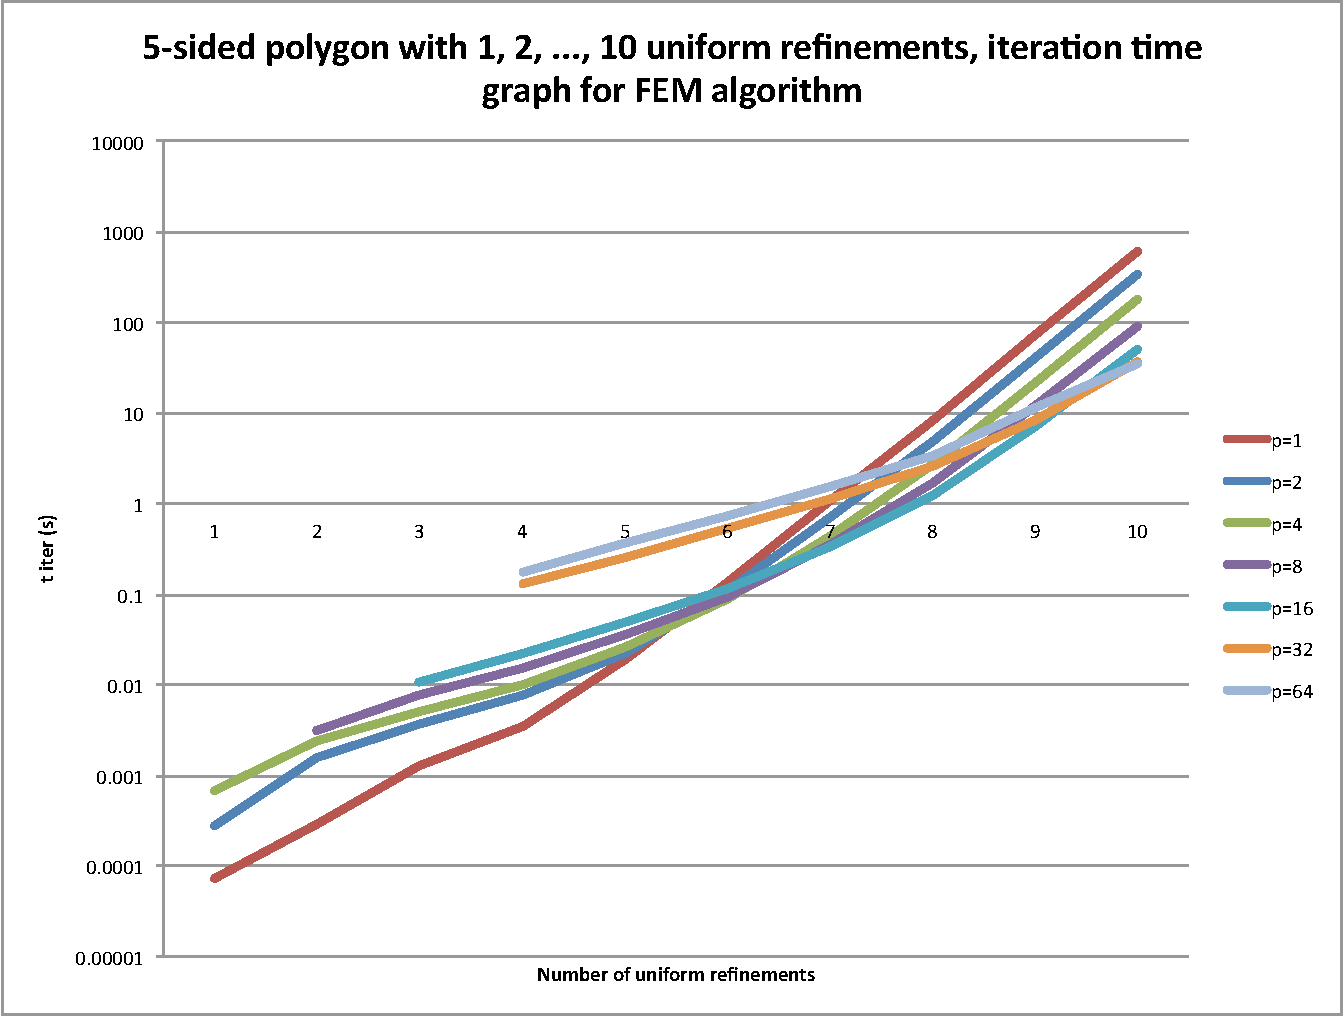
\includegraphics[width=0.8\linewidth]{times_fem.pdf}
  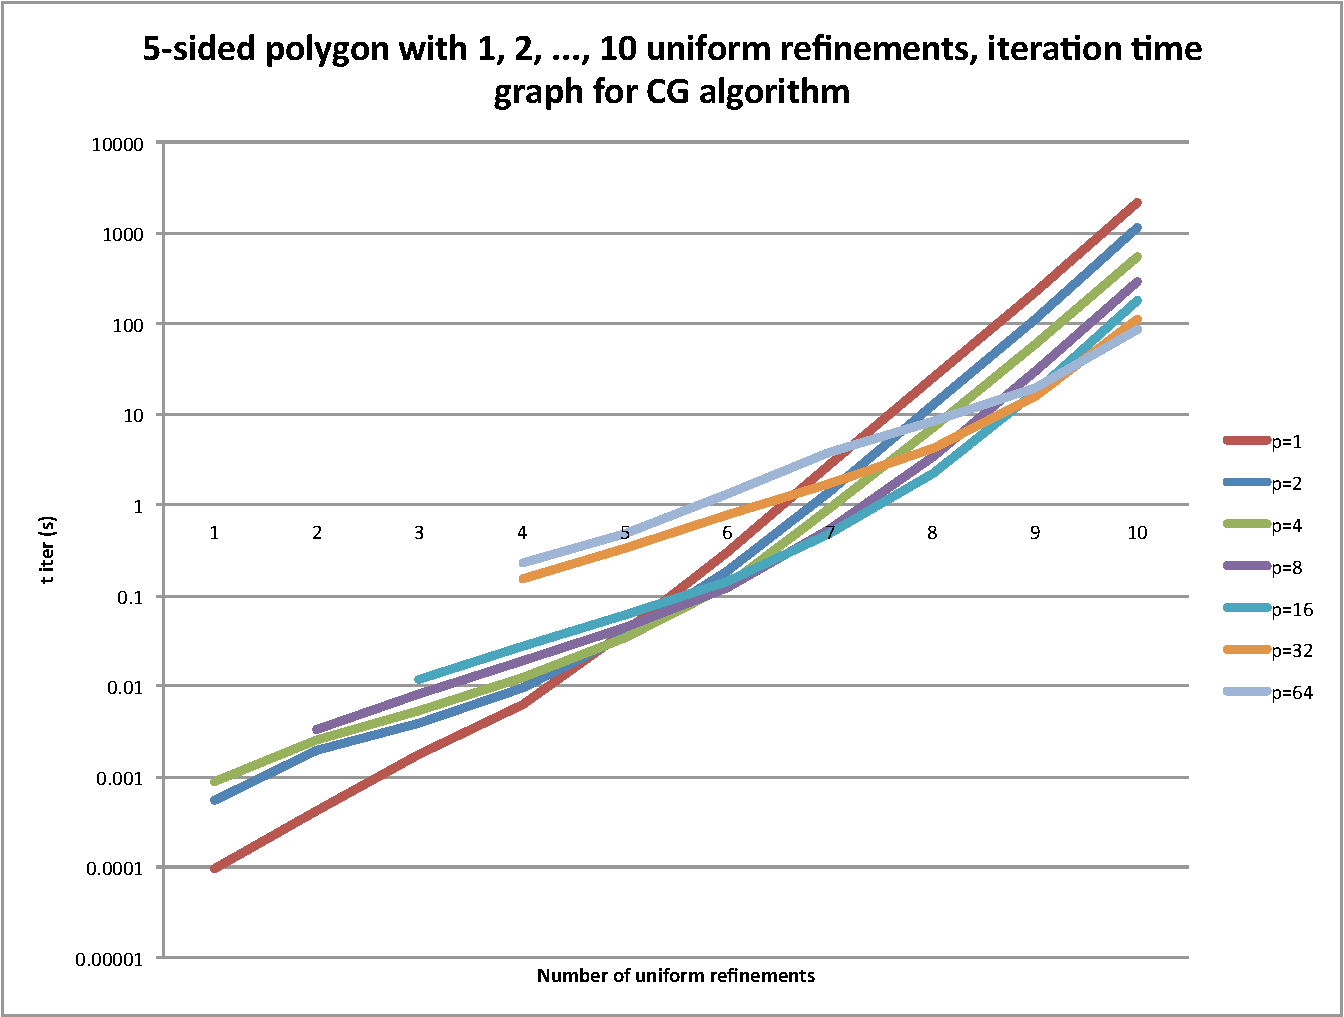
\includegraphics[width=0.8\linewidth]{times_cg.pdf}
  \caption{We see that parallelization does not make sense for systems that are too small.}
  \label{fig:times}
\end{figure}

Let's look at a small system where parallelization is of no use. We take $n=5$, and leave out $p \in \{32,64\}$ as these are orders of magnitude slower. See Figure~\ref{fig:barchart_oud}. Something that is immediately clear, is that $t_{ip}$ increases exponentially in $p$ while $t_{mv}$ and $t_{init}$ change in a much less defined manner. This is because of the small computation time and the large $h$-relation of the inner product.
\begin{figure}
  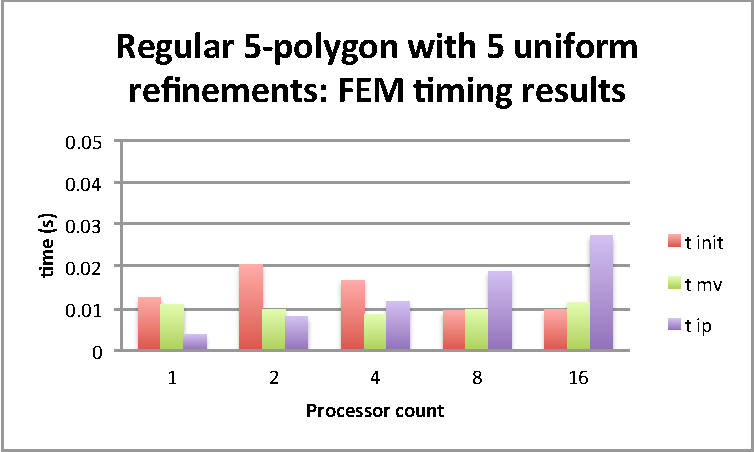
\includegraphics[width=0.48\linewidth]{barchart_oud_fem.pdf}
  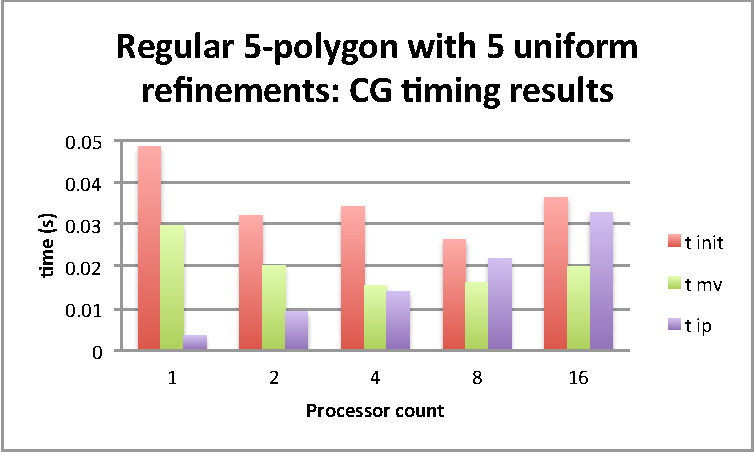
\includegraphics[width=0.48\linewidth]{barchart_oud_cg.pdf}
  \caption{Comparison between timing results of the different algorithms. Left: FEM algorithm; right: CG algorithm.}
  \label{fig:barchart_oud}
\end{figure}

We created a regular 5-polygon and made 10 uniform refinements, yielding 2.6M vertices and 5.2M triangles.\footnote{In fact, we even created a regular 8-polygon with 11 uniform refinements (which is 1.2G of mesh data alone), but for this system, we were unable to create a FEM matrix so no comparison with the original CG was possible.} Running this requires $k=4352$ iterations. We will discuss Figure~\ref{fig:baazen}. One thing we see is that in both algorithms, 
\begin{itemize}
  \item[-] $t_{init}$ seems more or less invariant under the processor count; 
  \item[-] $t_{mv}$ is the most substantial step;
  \item[-] $t_{ip}$ decreases in $p$ for $p < 24$ and increases there-after;
  \item[-] $t_{ip}$ is more or less the same for both algorithms;
  \item[-] If we were to look at higher processor counts, $t_{ip}$ will get the overhand (we already saw this happening far earlier with smaller systems).
\end{itemize}
The main difference is the fact that $t_{mv}$ is a factor 4 faster in the new case versus the old case.\footnote{This has to do with the fact that the two matrix-vector algorithms are different: (1) we exploit the geometrical information of the FEM system, thereby needing less communication and not needing the fanout superstep, (2) the matrix-vector product is now symmetric, avoiding cache misses.} The total speedup factor is around 3. If we look at disk storage, the new algorithm requires around a factor 6 less storage space (saving meshes versus systems).

\begin{figure}
  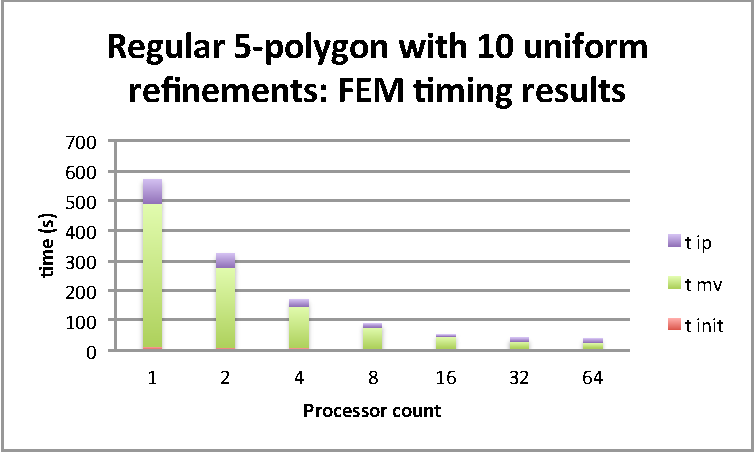
\includegraphics[width=0.48\linewidth]{baazen_fem.pdf}
  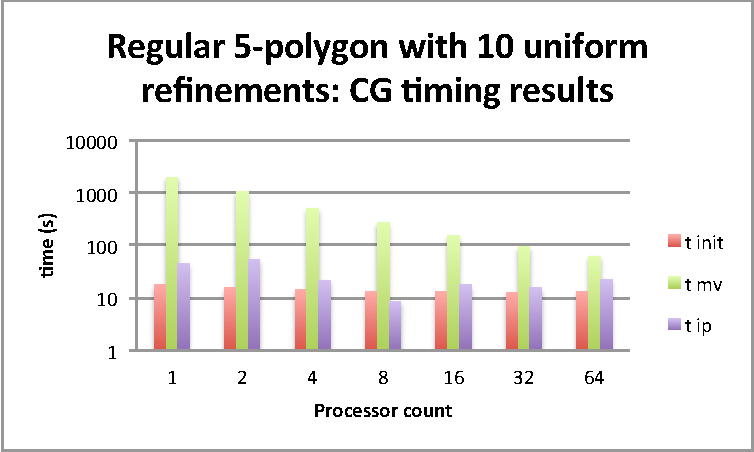
\includegraphics[width=0.48\linewidth]{baazen_cg.pdf}
  \caption{Taking a regular 5-polygon with 10 uniform refinements (for a total of $N = 5.2$M triangles and $D = 2.6$M degrees of freedom). Left: timing results for our FEM implementation. Right: original CG implementation.}
  \label{fig:baazen}
\end{figure}

\section{Conclusion}
In this report we have developed two parallel CG algorithms for solving $Ax =b$, with $A$ a sspd matrix. The first algorithm works by defining a distribution for the nonzeros of $A$. We then use \verb=bspmv= and a slightly altered version of \verb=bspip= to create a parallel CG implementation. This version distributes the elements $A_{ij}$ and therefore works for any sspd matrix.
We have tested this method for a set of random generated matrices. Unfortunately, our method of matrix generation had some deficiencies. The matrices it produces are almost diagonal, which resulted in distorted timing results: the CG method converges really quick, and we do not benefit from parallelizing.

In the second part we looked at a specific class of sspd matrices, namely the stiffness matrices comming from FEM systems. After creating such a method we can use the parallel CG method from the first part to solve the FEM-system $Ax = b$. This works by creating the stifness matrix $A$ and then using Mondriaan to find a distribution for the non-zero elements.

As we are looking at FEM-matrices we have additional information available about the matrix $A$. We can use the fact that the matrix is related to a triangulation of the domain. If we distribute the triangles of this trianuglation over the processors, we are able to give another way of calculating the matrix-vector product $u = Av$ and the inner product $\langle u, v \rangle$.  This approach  is different from traditional methods, in the sense that multiple processors will have to maintain a copy of certain data. 

We can use our triangle distribution and the according matrix- and vector-operations for implementing parallel CG. Using a distribution given by Mondriaan, we have tested and compared both methods. We saw that small FEM-system do not benefit from parallelizing. Once the systems become large however, we saw a vast speed-up in both methods when comparing sequential with the parallel version. Also, the parallel FEM cg method presented in the second part was about $2$ to $4$ times faster than the initial parallel CG method.

\section{Discussion}
Initially we worked out Exercise~4.6 from \cite{biss04}. We gathered a lot of results for different densities, $n$ and processor counts. After processing these results, we came to the conclusion that most of this data was not representative for the actual performance of the parallel CG algorithm. This comes from the fact that the matrices created are \emph{really} strictly diagonally dominant, in other words, they are almost diagonal matrices. This causes CG to converge in a low amount of iterations, which results in a really small speed-up from parallelizing.
A suggestion for the exercise might be to gather matrices from the Matrix Market, or to use our FEM-matrices.

We wanted to work on FEM-matrices, as we have both done something with FEM in the past of our academic career.\footnote{We actually got to use this method and our previous work, which is really cool. See \cite{TODOCITES}.} Clearly, these matrices provide better input for testing the parallel CG. Comparing the second method with the first method, we actually saw a nice speed-up. Again, we generated a lot of data for several triangulations and its uniform refinements. When processing the data, we again did not see a big speed-up in parallelizing. When writing the report we came to the conclusion that the systems we tested were too small. So last-minute we generated some enourmous triangulations and recreated all the timings. Here we finally saw the speed-up of parallelizing.

\section{Future work}
During the project we came up with a lot of interesting stuff we could have figured out. Here we have a summary of things we could improve our work with.
\subsection{Inner product}
For large systems we saw that the time spent in matrix-vector products reduces when using more processors, whilst the time spent in the inner product actually increases. We want to figure out if we could possibly improve the time of the inner product. An example would be demanding other properties from the triangle distribution. Another idea is to use one or two passes from the method proposed in the first Homework exercise before switching to the old method.
\subsection{Preconditioned CG}
The iterates $x_k$ obtained from the CG algorithm satisfy the following inequality \cite[Lect.~7]{sleij}:
\[
  \frac{\|x - x_k\|_A}{\|x - x_0\|_A} \leq 2 \left( \frac{ \sqrt{\kappa_2(A)}-1}{\sqrt{\kappa_2(A)}+1}\right)^k \leq 2 \exp \left( -\frac{2k}{\sqrt{\kappa_2(A)}}\right) 
\]
where $\kappa_2(A)$ is the $2$-condition number of $A$, which for spd matrices equates
\[
  \kappa_2(A) = \frac{\lambda_{max}}{\lambda_{min}}.
\]
It is therefore of interest to create a condition number that is as low as possible.

A preconditioner $P$ of a matrix $A$ is a matrix such that $P^{-1}A$ has a smaller condition number than $A$. As the theoretical convergence rate is highly dependent on the condition number, we can improve this using such a preconditioner. Instead of solving $Ax = b$, we will solve $P^{-1}Ax = P^{-1}b$. This preconditioner should satisy:
\begin{itemize}
  \item Convergence time should be faster for the preconditioned system. Normally, this means that $P$ is constructed as an ``easily invertible'' approximation to $A$;
  \item Operations with $P^{-1}$ should be easy to perform;
  \item $P$ should be (relatively) easy to construct.
\end{itemize}

If $A$ is positive definite, the diagonal tells us a lot about the properties of $A$ so it makes a certain amount of sense to consider perhaps the simplest preconditioner of all:
\[
  P = \text{diag}(a_{11}, \ldots, a_{nn}).
\]
The beauty of this preconditioner is the fact that its sparsity pattern is just like a dense vector. Therefore, given a vector distribution (like we already have in our implementation), creating a preconditioned version is easy. We did not have time to implement this, unfortunately.

A more advanced preconditioner that is often used in the spd case is Incomplete Cholesky.  The Cholesky factorization of a positive definite matrix $A$ is $A = LL^*$ with $L$ a lower triangular matrix. An incomplete Cholesky factorization is any sparse lower triangular $K$ that is in some sense close to $L$. One such $K$ can be found by finding the exact Cholesky decomposition, except that any entry is set to zero if the corresponding entry in $A$ is also zero. \cite[\S11.5.8]{golub}
\subsection{Adaptive FEM}
Another interesting aspect one could look at is adaptive FEM.
Popularly speaking, adaptive FEM aims to improve the quality of the FEM-solution $u_V$ by locally refining the triangulation. This implies that only a part of the stiffness matrix will have to be recalculated. A few interesting things to look at would be:
\begin{itemize}
	\item Ensure each processor autonomously refines its own part of the triangulation;
	\item Make a load imblanace treshold that rebalances the entire triangulation after a few local refinements.
\end{itemize}
\subsection{Triangle distributions}
As described before, Mondriaan does not yet implement all the properties we want to use when partitioning a hypergraph. For better control of the triangle distributions one could look at other partitioners, for example PaToH. \cite{patoh}
\bibliographystyle{alpha}
\bibliography{report}

\end{document}
